 % reset section counter
%\setcounter{section}{0}
\metadata{8}{David Lin and Jinhui Wang}{Feb.~8th, 2021}

\sec{Covering number upper bounds Rademacher complexity}
In Chapter \ref{chap:gen-bounds}, we will prove Rademacher complexity bounds that hinge on elegant, ad-hoc algebraic manipulations that may not extend to more general settings. Here, we consider a more fundamental approach for proving empirical Rademacher complexity bounds based on coverings of the output space. The trade-off is generally more tedium.

The first important observation is that for purposes of computing the \textbf{empirical} Rademacher complexity on samples $z_1, ..., z_n$, 
\al{
    R_S(\cF) = \E_\sigma \sbr{\sup_{f \in \cF} \frac 1 n \sum_{i=1}^n \sigma_i f(z_i)},
}
we only care about each function's $f \in \cF$ behavior on $\{z_1, ..., z_n\}$. Hence, we can forget the rest of the input space and characterize $f \in \cF$ by its outputs $(f(z_1),\dots, f(z_n))$. Thus, there is a paradigm shift from the space of all functions $\cF$ to the \textit{output space}
\begin{equation}
\cQ \triangleq \cbr{ \begin{pmatrix} f(z_1), \dots, f(z_n) \end{pmatrix}^\top: f\in \cF} \subseteq \R^n,
\end{equation}
which may be drastically smaller than $\cF$. Correspondingly, the empirical Rademacher complexity can be rewritten as a maximization over the output space $\cQ$ instead of the function space $\cF$: 
\al{
    R_S(\cF) &= \E_\sigma \sbr{\sup_{v\in \cQ} \frac 1 n \inprod{\sigma, v}}.
}
In other words, the complexity of $\cF$ can be also interpreted as how much the vectors in $Q$ can be correlated with a random vector $\sigma.$ See Figure \ref{lec6:fig:rs-innerprod} for an illustration of this idea. One can also view $\E_\sigma \sbr{\sup_{v\in \cQ} \frac 1 n \inprod{\sigma, v}}$ as a complexity measure for the set $Q$. If we replace $\sigma$ by a Gaussian vector with spherical covariance, then the corresponding quantity (without the $\frac 1 n$ scaling), $\E_{g\sim N(0,I)} \sbr{\sup_{v\in \cQ} \inprod{g, v}}$, is often referred to as the Gaussian complexity of the set $Q$. (It turns out that Gaussian complexity and Rademacher complexity are closely related.)

Another corollary of this is that the empirical Rademacher complexity only depends on the functionality of $\cF$ but not on the exact parameterization of $\cF$ . For example, suppose we have two parameterizations $\cF = \left\{f(x)=\sum \theta_{i} x_{i} \mid \theta \in \mathbb{R}^{d}\right\}$ and $\cF' = \left\{f(x)=\sum \theta_{i}^{3} \cdot w_{i} x_{i} \mid \theta \in \R^{d}, w \in \mathbb{R}^{d}\right\}$. Since $Q_\cF$ and $Q_{\cF'}$ are the same, we see that $R_S(\cF) = R_S(\cF')$ since our earlier expression for $R_S(\cF)$ only depends on $\cF$ through $Q_\cF$. 

\tnoteimp{replace backslash E by backslash Exp in all displayed equations in all files; (I think it's perhaps even okay to replace in all occurrences because for inaligned texts I think they are the same? Need to be checked)}

\begin{figure}[ht!]
	\begin{center}
		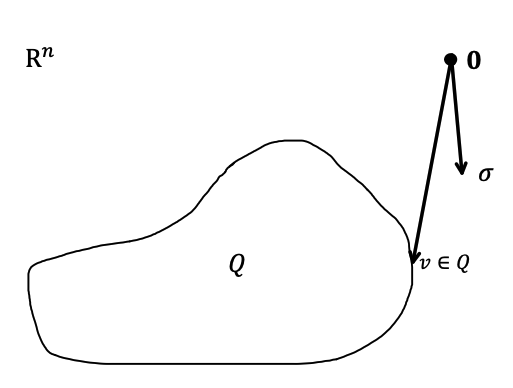
\includegraphics[width=.5\textwidth]{figures/remark2.png}
	\end{center}
	\caption{We can view empirical Rademacher complexity as the expectation of the maximum inner product between $\sigma$ and $v\in Q$.}
	\label{lec6:fig:rs-innerprod}
\end{figure}

\paragraph{Rademacher complexity of finite hypothesis class.} Now, for finite $|\cQ|$, we immediately obtain the following bound by Massart's lemma: \tnoteimp{I realize that we didn't have the Massart lemma formally in the lecture notes. Could you add it here with some transition texts, John? You can perhaps reuse the equations in homework (where they are asked to prove the Massart lemma)}
\begin{equation}
R_S(\cF) \le \sqrt{\frac {2\log|\cQ|} n}.
\end{equation}
\paragraph{Bounding Rademacher complexity using $\epsilon$-cover }
When $|\cQ|$ is infinite, we can use the same discretization trick that we used to prove the generalization bound for an infinite-hypothesis space. Instead of trying to cover the parameter space, we try to cover the output space. To this end, we firstly recall a few definitions concerning $\epsilon$-covers.

\begin{definition}
$\cC$ is an \emph{$\epsilon$-cover} of $\cQ$ with respect to metric $\rho$ if for all $v\in \cQ$, there exists $v'\in \cC $ such that $\rho(v,v')\le \epsilon$.
\end{definition}

\begin{definition}
The \emph{covering number} is defined as the minimum size of an $\epsilon$-cover, or explicitly:
$$N(\epsilon, \cQ, \rho) \overset \triangle = (\text{min size of $\epsilon$-cover of $\cQ$ w.r.t.\ metric $\rho$}).$$
\end{definition}

The standard metric we will use is $\rho(v,v') = \frac 1 {\sqrt{n}} \norm{v-v'}_2$, with the leading coefficient inserted for convenience.

\begin{remark}
While we want to consider $\epsilon$-covers over $\cQ$, the notation in the literature refers to them as $\epsilon$-covers of the function class $\cF$ using the metric $\rho = L_2(p_n)$, i.e.
\begin{equation}
\rho(f,f') = \sqrt{ \frac 1 n \sum_{i=1}^n (f(z_i) - f'(z_i))^2 }
\end{equation}
If we take the corresponding $v,v'\in \cQ$, this is precisely $\rho(v,v') = \frac 1 {\sqrt{n}} \norm{v-v'}_2$.
\end{remark}

Equipped with the notion of $\epsilon$-covers, we can prove the following Rademacher complexity bound:

\begin{theorem}\label{lec8:thm:rc-covering-bd}
Let $\cF$ be a family of functions $Z \mapsto [-1,1]$. Then
\begin{equation}
R_S(\cF) \le \inf_{\epsilon > 0} \rbr{ \epsilon + \sqrt{ \frac {2\log N(\epsilon, \cF, L_2(P_n))} n } }. \label{lec8:eqn:rc-covering-bd}
\end{equation}
\end{theorem}

The $\epsilon$ term can be thought of as the discretization error, while the latter term is the term from Massart's lemma.

\begin{proof}
Fix any $\epsilon > 0$. Let $\cC$ be an $\epsilon$-cover $\cC$ of $\cQ$. Massart's lemma immediately gives the bound
\al{
R_S(\cC) \le \sqrt{ \frac {2\log |\cC|} n }.
}
For every point $v\in \cQ$, we can express it as $v=v'+z$, where $v'\in \cC$ and $z$ is small (specifically, $\frac 1 {\sqrt{n}} \norm{z}_2 \le \epsilon$). This gives
\al{
    \frac 1 n \inprod{v, \sigma} &= \frac 1 n \inprod{v',\sigma} + \frac 1 n \inprod{z, \sigma}\\
    &\le \frac 1 n \inprod{v', \sigma} + \frac 1 n \norm{z}_2 \norm{\sigma}_2 
        &&\text{(Cauchy-Schwarz)} \label{lec8:eqn:cs-step}\\
    &\le \frac 1 n \inprod{v', \sigma} + \epsilon.
        &&\text{(since $\norm{z}_2\le \sqrt{n}\epsilon$ and $\norm{\sigma}_2 \le \sqrt{n}$)}
}
Taking the expectation of the supremum on both sides of this inequality gives
\al{
    R_S(\cF) &= \E_\sigma \sbr{\sup_{v\in \cQ} \frac 1 n \inprod{v,\sigma} }\\
    &\le \E_\sigma \sbr{\sup_{v'\in \cC} \rbr{\frac 1 n \inprod{v',\sigma} + \epsilon}}\\ 
    &\le \sqrt{ \frac {2\log \abs{\cC}} n } + \epsilon. &\text{(Massart's lemma)}
}
Choosing $\cC$ to be a minimal $\epsilon$-cover allows us to set $|\cC| = N(\epsilon, \cF , L_2(p_n))$. Since the argument above holds for any $\epsilon > 0$, we can take the infimum over all $\epsilon$ to arrive at Equation \eqref{lec8:eqn:rc-covering-bd}, completing the proof.

\end{proof}

\sec{Chaining and Dudley's theorem}

While Theorem \ref{lec8:thm:rc-covering-bd} is useful, the bound in Equation \eqref{lec8:eqn:cs-step} is rarely tight as $z$ might not be perfectly correlated with $\sigma$. It is possible to obtain a stronger theorem by constructing a chained $\epsilon$-covering scheme. Specifically, when we decompose $v=v'+z$, we can construct a finer-grained covering of the ball $B(v',\epsilon)$, and then we can decompose $z$ into smaller components and so on (see Figure \ref{lec8:fig:chained cover} for an illustration).

\begin{figure}[H]
    \centering
    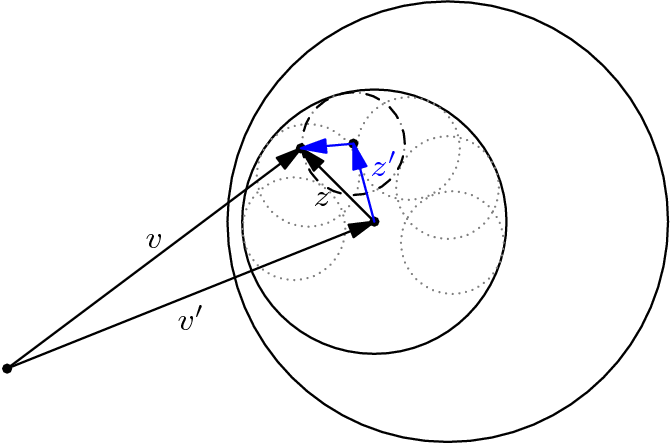
\includegraphics[scale = 0.4]{figures/chaining.png}
    \caption{Illustration of a chained cover. Within the $\epsilon$-ball containing the discretization error $z$, we find a finer $\epsilon'$-cover and obtain a smaller error $z'$ from discretizing $z$.}
    \label{lec8:fig:chained cover}
\end{figure}

Using this method of chaining, we can obtain the following (stronger) result:

\begin{theorem}[Dudley's Theorem]
If $\cF$ is a function class from $Z$ to $\R$, then

\begin{equation}\label{lec9:eqn:dudley}
    R_S(\mathcal{F})\leq 12\int_{0}^{\infty}\sqrt{\frac{\log N(\epsilon, \mathcal{F}, L_2({P_n}))}{n}}d\epsilon.
\end{equation}

\end{theorem}

We can interpret this bound as removing the discretization error term by averaging over different scales of $\epsilon$. For a proof of this theorem, refer to Theorem 15 of \cite{percynotes}.

If $\mathcal{F}$ consists of functions bounded in $[-1,1]$, then, we have that for all $\epsilon > 1, N(\epsilon, \mathcal{F}, L_2({P_n}))=1$. (To see this choose $\{f\equiv 0\}$, which is a complete cover for $\epsilon>1$.) Hence, the limits of integration in \eqref{lec9:eqn:dudley} can be truncated to $[0,1]$:
    
    \begin{equation}
    R_S(\mathcal{F})\leq 12\int_{0}^{1}\sqrt{\frac{\log N(\epsilon, \mathcal{F}, L_2({P_n}))}{n}}d\epsilon,
    \end{equation}
    
since $\log N(\epsilon, \mathcal{F}, L_2(P_n))=0$ for $\epsilon >1$.

\subsec{Covering number regimes for which Dudley's theorem is finite}

Of course, the bound in \eqref{lec9:eqn:dudley} is only useful if the integral on the RHS is finite. Here are some setups where this is the case (we continue to assume that the functions in $\cF$ are bounded in $[-1, 1]$):

\begin{enumerate}
\item If $N(\epsilon, \mathcal{F}, L_2(P_n))\approx (1 / \epsilon)^R$ (ignoring multiplicative and additive constants), then we have $\log N(\epsilon, \mathcal{F}, L_2(P_n))\approx  R\log (1/\epsilon)$. We can plug this into the RHS of \eqref{lec9:eqn:dudley} to get
        
\begin{equation}
\int_{0}^{1}\sqrt{\frac{\log N(\epsilon, \mathcal{F}, L_2({P_n}))}{n}}d\epsilon = \int_{0}^1\sqrt{\frac{R\log(1/\epsilon)}{n}}d\epsilon \approx \sqrt{\frac{R}{n}}.
\end{equation}
            
\item If the covering number has the form $N(\epsilon, \mathcal{F}, L_2(P_n))\approx a^{R/\epsilon}$ for some $a$, then we have $\log N(\epsilon, \mathcal{F}, L_2(P_n)) \approx \frac{R}{\epsilon}\log a$. The bound in \eqref{lec9:eqn:dudley} becomes
        
\begin{align}
\int_0^1\!\!\sqrt{\frac{\log N(\epsilon, \mathcal{F}, L_2(P_n))}{n}}d\epsilon &\approx \int_0^1\!\!\sqrt{\frac{R}{n\epsilon}\log a}\, d\epsilon \\
&= \sqrt{\frac{R}{n}\log a} \int_0^1\!\!\sqrt{\frac{1}{\epsilon}}d\epsilon \\
&= \tilO \l(\sqrt{\frac{R}{n}}\r).
\end{align}
        
\item If the covering number has the form $N(\epsilon, \mathcal{F}, L_2(P_n))\approx a^{R/\epsilon^2}$, then $\log N(\epsilon, \mathcal{F}, L_2(P_n))\approx \frac{R}{\epsilon^2}\log a$. In this case we have:
        
\begin{equation}\int_0^1\sqrt{\frac{\log N(\epsilon, \mathcal{F}, L_2(P_n))}{n}}d\epsilon \approx \sqrt{\frac{R}{n}\log a} \underbrace{\int_0^1\frac{1}{\epsilon}d\epsilon}_{=\infty}=\infty,
\end{equation}

i.e. the bound in \eqref{lec9:eqn:dudley} is vacuous. This is because of the behavior of $\epsilon \mapsto 1/\epsilon^2$ near 0: the function goes to infinity too quickly for us to upper bound its integral. Fortunately, there is an ``improved'' version of Dudley's theorem that is applicable here:
        
\begin{theorem}[Improved Dudley's Theorem]\label{lec9:thm:better-dudley}
If $\cF$ is a function class from $Z$ to $\R$, then for any fixed cutoff $\alpha \geq 0$ we have the bound
\begin{equation}\label{lec9:eqn:better-dudley}
R_S(\mathcal{F})\leq 4\alpha + 12\int_{\alpha}^{\infty}\sqrt{\frac{\log N(\epsilon, \mathcal{F}, L_2({P_n}))}{n}}d\epsilon.      
\end{equation}
\end{theorem}
The proof of this theorem is similar to the proof of the original Dudley's theorem, except that the iterative covering procedure is stopped at the threshold $\epsilon = \alpha$ at the cost of the extra $4\alpha$ term above.
        
Theorem \ref{lec9:thm:better-dudley} allows us to avoid the problematic region around $\epsilon=0$ in the integral in \eqref{lec9:eqn:dudley}. If we let $\alpha = 1/poly(n)$, the bound in \eqref{lec9:eqn:better-dudley} becomes
        
\begin{align}
R_S(\mathcal{F}) &\leq \frac{1}{poly(n)} + \frac{\sqrt{R\log a}}{\sqrt{n}}\int_{\alpha}^1\frac{1}{\epsilon}d\epsilon \\
&= \frac{1}{poly(n)}  + \frac{\sqrt{R\log a}}{\sqrt{n}} \log(1/\alpha) \\
&= \tilO \l(\sqrt{\frac{R}{n}}\r).
\end{align}
\end{enumerate}

In summary, we have that $R_S(\mathcal{F}) \leq \tilO\l(\sqrt{\frac{R}{n}}\r)$ for these three dependencies on $\epsilon$: when $\log N(\epsilon, \mathcal{F}, L_2({P_n})) \approx R\log (1/\epsilon),\ \frac{R}{\epsilon} \log a,\text{ or } \frac{R}{\epsilon^2} \log a$ for some $a$. Note that if the dependence on $\epsilon$ is $1/\epsilon^c$ for $c > 2$, then even the improved Dudley's theorem does not help us. This is because the $\log(1/\alpha)$ term above becomes $\alpha^{1-c/2}$, and when $\alpha = 1/poly(n)$, this term leads to a bad dependence on $n$.

\subsec{Regimes where we can get covering number bounds}
The previous remarks discuss how strong our bounds on covering number need to be in order to get a useful result. Here we mention some situations in which we know how to obtain these covering number bounds:

\begin{enumerate}
\item Covering number and corresponding Rademacher complexity bounds for linear models are well-known, but fairly technical (see \cite{zhang2002}).
    
\item Covering numbers interact nicely with composition by Lipschitz functions. If $\phi$ is a $\rho$-Lipschitz function, then the following bound holds:
\begin{equation}\label{lec9:eqn:covering-num-lipschitz}
N(\epsilon/\rho, \mathcal{F}, L_2({P_n}))\geq N(\epsilon, \phi\circ\mathcal{F}, L_2({P_n})).
\end{equation}
    
This result is the analog of Talagrand's lemma for covering numbers. The proof follows easily if one considers $\phi$ as a change of measure: informally, the Lipschitz condition on $\phi$ means that a distance of $\epsilon/\rho$ in the original space $\mathcal{F}$ can be increased to at most $\epsilon$ in the space $\phi \circ \mathcal{F}$.

\item Using these results we can obtain a bound on the Rademacher complexity of a dense neural network. Consider a deep network
\begin{equation}
f(x) = W_r\sigma(W_{r-1}\sigma(\cdots \sigma(W_1x)\ldots),
\end{equation}

where $W_i$ are layer-wise weights and $\sigma$ is an activation function which is 1-Lipschitz. For this setup we have the following Rademacher complexity bound:
\begin{equation}
R_S (\cF) \leq \underbrace{\l(\prod_{i=1}^r\|W_i\|_{\textup{op}} \r)}_{\text{relatively large}} \cdot \underbrace{\l( \sum_{i=1}^r\frac{\|W_i^\top\|^{2/3}_{2,1}}{\|W_i\|_{\textup{op}}^{2/3}}\r)^{3/2}}_{\text{relatively small}}.
\end{equation}
        
Here $\|W\|_{\textup{op}}$ is the operator norm (or spectral norm) of $W$, and $\|W_i^\top\|_{2,1}$ denotes the sum of the $l_2$ norms of the rows of $W_i$. The second term is relatively small as it is a sum of matrix norms, and so the bound is dominated by the first term, which is a product of matrix norms. This first term comes from composition of Lipschitz functions as in \eqref{lec9:eqn:covering-num-lipschitz} above, since the Lipschitz constant of a linear operator is its spectral norm. The full details are presented in \cite{bartlett2017}.
\end{enumerate}


\sec{VC dimension and its limitations}
We will focus on classification and will be working within the framework of supervised learning stated in Chapter \ref{chap:supervised}. The labels belong to the output space $\mathcal{Y} = \{-1, 1\}$, each classifier is a function $h:\mathcal{X}\to\R$ for all $h \in \cH$, and the prediction is the sign of the output, i.e. $\hat{y} = \sgn(h(x))$. We will look at zero-one loss, i.e. $\err((x,y), h) = \mathbbm{1}(\sgn(h(x))\neq y)$. Note that we can re-express the loss function as
\begin{equation}
\err((x,y), h) = \frac{1-\sgn(h(x))y}{2}.
\end{equation}

The first approach is to reason directly about the Rademacher complexity of $\err$ loss, i.e. considering the family of functions $\cF = \left\{ z = (x, y) \mapsto \err((x, y), h) : h \in \cH \right\}$. Define $Q$ to be the set of all possible outputs on our dataset: $Q=\left\{\left(\sgn\left(h\left(x^{(1)}\right)\right), \dots, \sgn \left(h\left(x^{(n)}\right)\right)\right)\mid  h \in \cH \right\}$. Then, using our earlier remark about viewing the empirical Rademacher complexity as an inner product between $v\in Q$ and $\sigma$, we have
\begin{align}
R_S(\cF) &= \E_{\sigma_1,\dots, \sigma_n} \l[ \sup_{f\in \cF} \frac{1}{n} \sum^n_{i=1} \sigma_i \frac{1-\sgn(h(x^{(i)}))y_i}{2} \r] \\
&= \E_{\sigma_1,\dots, \sigma_n} \l[ \sup_{f\in \cF} \frac{1}{n} \sum^n_{i=1} \sigma_i \frac{\sgn(h(x^{(i)}))}{2} \r] \\
&= \frac{1}{2}\E_{\sigma_1,\dots, \sigma_n} \l[ \sup_{v\in Q} \frac{1}{n} \langle \sigma, v\rangle \r].
\end{align}

Notice that the supremum is now over $Q$ instead of $\cF$. If $n$ is sufficiently large, then it is typically the case that $|Q|>|\cF|$. To see why this is the case, note that each function $f$ corresponds to a single element in $Q$. However, as $n$ increases, $|Q|$ increases as well. For any particular $v\in Q$, notice that $\langle v, \sigma\rangle$ is a sum of bounded random variables, so we can use Hoeffding's inequality to obtain
\begin{equation}
\Pr\left[\frac{1}{n}(\sigma, v) \geq t\right] \leq \exp (-n t^2 / 2).
\end{equation}
Taking the union bound over $v\in Q$, we see that 
\begin{equation}
\Pr\left[\exists v\in Q \text{ such that } \frac{1}{n}\langle\sigma, v\rangle \geq t\right] \leq |Q| \exp (-nt^2 / 2).
\end{equation}
Thus, with probability at least $1-\delta$, it is true that $\sup _{v \in Q} \frac{1}{n}\langle v, \sigma \rangle \leq \sqrt{\frac{2(\log|Q| + \log (2/\delta))}{n}}$. Similarly, we can show that $\E \left[ \sup _{v \in Q} \frac{1}{n}\langle v, \sigma \rangle \right] \leq O\l(\sqrt{\frac{\log|Q| + \log (2/\delta)}{n}}\r)$ holds.

The key point to notice here is that the upper bound on $R_S(\cF)$ depends on $\log |Q|$. \textit{VC dimension} is one way that we deal with bounding the size of $Q$ We will not delve into the details of this approach (for those interested, see Section 3.11 of \cite{percynotes}). VC dimension, however, has a number of limitations. For one, we will always end up with a bound that depends somehow on the dimension. For linear models, we obtain a bound $\log |Q| \lesssim d \log n$, corresponding to a bound on Rademacher complexity that looks like
\begin{equation}
R_S(\cF) \leq \tilO \left( \sqrt{\frac{d}{n}} \right),
\end{equation}
so we still have a $\sqrt{d}$ term. This will not be a good bound for high-dimensional models. For general models, we will arrive a bound of the form 
\begin{equation}
R_S(\cF) \leq \tilO \left( \sqrt{\frac{\text{\# of parameters}}{n}} \right).
\end{equation}
This upper bound only depends on the number of parameters in our model, and does not take into the account the scale and norm of the parameters. Additionally, this doesn't work with kernel methods since the explicit parameterization is possibly infinite-dimensional, and therefore this upper bound becomes useless.

These limitations motivation the use of margin theory, which does take into account the norm of parameters and provides a theoretical basis for regularization techniques such as $L_1$ and $L_2$ regularization.